\chapter{绪论}
相变是凝聚态物理学的核心内容之一,其描述了系统在外部参数变化时从一种物理相向另一种相的突变。
朗道相变理论(Landau Phase Transition Theory)是由苏联物理学家朗道(Lev Landau)提出的一种描述相变的唯象理论\cite{landau1937theory,landau1980statistical}。
在朗道相变理论中,相变是序参量及其导数和高阶导数的不连续行为。
这种不连续性,是系统对称性破缺的结果。
朗道相变理论通过对称性破缺和自由能的极小化原理,系统地解释了相变机制。
尽管朗道相变理论成功地描述了广泛的相变现象,但它本质上局限于对称性破缺驱动的相变。
随着对量子材料理解的深入,朗道相变理论的局限性逐渐显现,促使拓扑相变等新概念的提出。

拓扑相变是一类不同寻常的相变,其特征不是对称性破缺或局部序参量,而是全局拓扑不变量的变化。
1980年,冯·克利青(Klaus von Klitzing)在实验中发现了整数量子霍尔效应(IQHE)\cite{klitzing1980new}。
这一效应揭示了系统的电导值由一个整数(拓扑不变量,即Chern数)决定,与传统的对称性破缺理论无关。
1982年,David J. Thouless及其合作者通过TKNN理论(Thouless, Kohmoto, Nightingale, and den Nijs)从拓扑数学的角度
解释了量子霍尔效应\cite{thouless1982quantized},首次将拓扑不变量引入凝聚态物理。
与传统相变不同,拓扑相变起源于系统波函数拓扑性质的变化,为相变行为提供了一种全新的视角。

1982年, 华人物理学家崔琦, 德国物理学家 Stormer发现横向电阻不仅可以取正整数, 还出现了 n=1/3 这样一个分数的平台\cite{tsui1982two},
标志着分数量子霍尔效应的发现。
1983年,劳克林(Laughlin)通过构造分数量子霍尔态的波函数成功解释了这一现象\cite{laughlin1983anomalous},首次提出了拓扑序的概念。
不同于传统的能带拓扑,分数量子霍尔效应是一种拓扑序现象,其起源于粒子之间的纠缠性质。
拓扑序将拓扑相的概念扩展到超越能带理论的领域,涵盖具有长程量子纠缠的物质相。
与对称性破缺相不同,拓扑序的特征是依赖于空间拓扑的基态简并性以及具有分数统计的奇异准粒子。
拓扑序为量子物质提供了更深层的理解,并因其拓扑态对局部扰动的鲁棒性而在容错量子计算中具有潜在应用。

本章主要介绍了拓扑相变的基本概念和基本原理,介绍量子霍尔效应,反常量子霍尔效应,分数量子霍尔效应,
谷霍尔效应以及高阶拓扑绝缘体等经典拓扑模型的发展脉络,以及其相应的拓扑不变量以及物理特性。
\section{拓扑绝缘体}
拓扑学是数学的一个分支,涉及在连续变形下保持的量。
在拓扑学中,封闭的表面可以平滑地变形为各种几何形状,而无需剪切和粘贴。
例如,图 \ref{fig:TopoGeo} 中的 6 个对象都有不同的几何结构,但只有三种不同的拓扑结构。
球体可以不断变为勺子,因此它们在拓扑上是等效的。
圆环和咖啡杯在拓扑上也是等价的,双圆环和茶壶也是如此。
这些不同几何的拓扑可以用Gauss-Bonnet定理描述,
\begin{equation}
	\frac{1}{2\pi}\int_{surface}KdA=2(1-g)
\end{equation}
它指出二维闭合表面的总高斯曲率 (K) 始终是一个整数。
这个拓扑不变量称为亏格 (g),描述了表面的拓扑结构,即内部的孔数。
拓扑不变量在系统的连续变形下保持不变。
具有相同拓扑不变量的对象在拓扑上是等效的;也就是说,它们处于相同的拓扑阶段。
只有在对象中创建或删除孔时,拓扑不变量才会更改。这个过程被称为拓扑相变。

\begin{figure}[htbp]
	\centering
	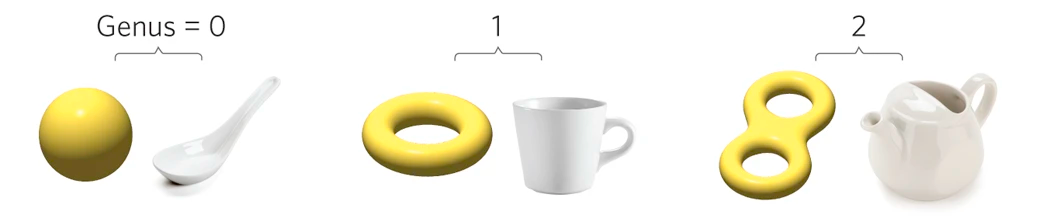
\includegraphics[width=0.75\textwidth]{TopoGeo.png}
 \caption{可以将 6 个不同几何图形的对象分组为三对拓扑。每对都有相同的拓扑不变量,称为其亏格。
图片来源于文献\cite{lu2014topological}}
 \label{fig:TopoGeo}
\end{figure}

拓扑绝缘体的拓扑结构则定义在倒易(波矢)空间的能带上。
二维布里渊区也是一个封闭表面,由于其周期性边界条件,它与环面具有相同的拓扑结构。
二维能带最经典的拓扑不变量是陈数,其用于表征波段上波函数的贝里相位的拓扑结构。
陈数是在圆环面上对 Berry 曲率的积分,它给出了 2D 表面的总量子化 Berry 通量的度量。
在这个圆环面上Berry磁通会产生一些单极子,它们是是贝里相位的奇点,可以类比为几何的孔洞。
因此陈数本质上就是这些单极子的数目,类似于亏格在前述几何中的定义。
此外,一旦物理可观测量可以写为类似的拓扑不变量,它就只会离散地改变。
因此,它不会响应连续的小扰动,这代表这其具有拓扑鲁棒性。

拓扑绝缘体最迷人的现象出现在边界。
如图\ref{fig:TopoBand}(a,b)所示,当界面两边的绝缘体具有相同的拓扑时,其沿着参数x连续变化不会有任何拓扑上的突变。
因此它们可以之间跨越能隙相连,无需关闭能隙。
而当界面两边具有不同拓扑时,连续变化参数x会在界面处出现能带拓扑的突变。
因此能带拓扑不会允许它们直接连接,必须在界面处闭合带隙以中和陈数。
而在此处闭合能隙的就是边缘态。
这些边缘态来源于界面两边不同的拓扑,因此它们是拓扑保护的。
边缘态的数目等于界面两边陈数的差异,这被称为体边对应,如图\ref{fig:TopoBand}(c)所示。
\begin{figure}[htbp]
	\centering
	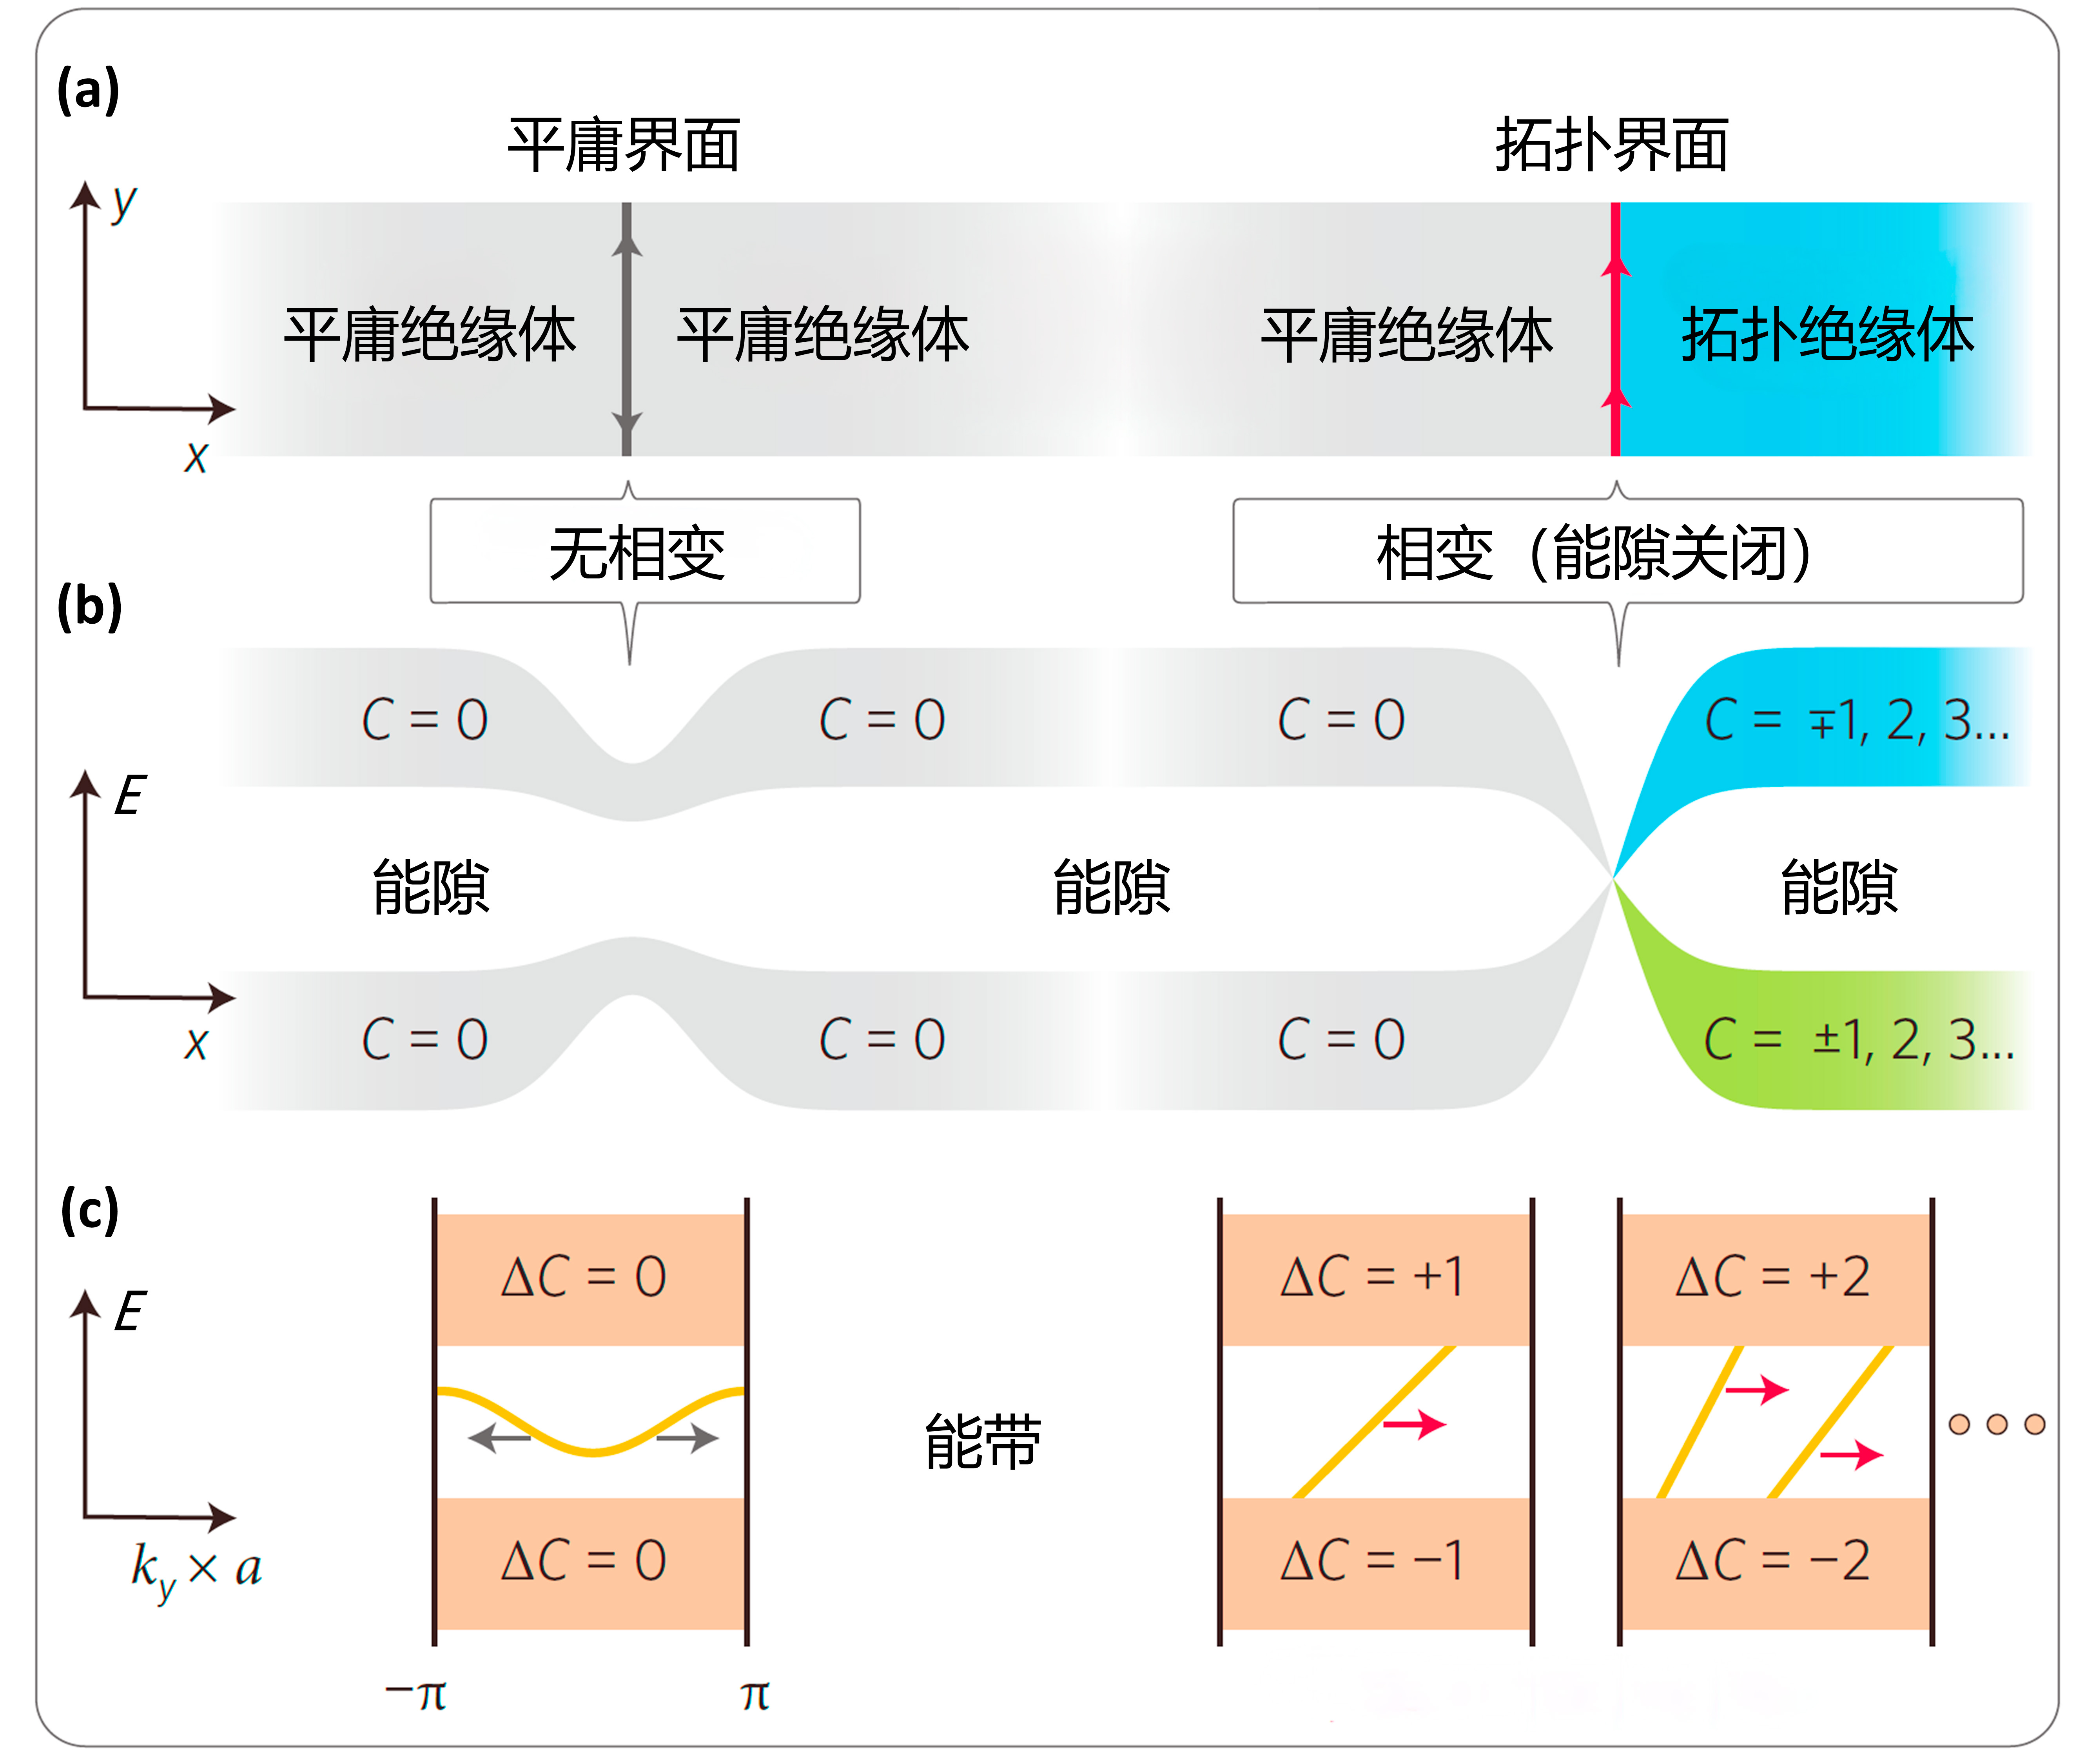
\includegraphics[width=0.75\textwidth]{TopoBand.jpg}
 \caption{(a)由不同(右)和相同(左)拓扑的绝缘体形成的两个界面。
(b)不同拓扑结构的频段如果不闭合带隙就无法相互过渡。
(c)界面态与体带具有不同的连通性,具体取决于绝缘体内的能带拓扑。
 其中,a 是波导沿y方向传播的周期,$\Delta C$是波导右侧和左侧相应体带之间陈数的变化。
 $\Delta C$的大小等于无间隙界面模式的数量,$\Delta C$的符号表示传播方向。
图片来源于文献\cite{lu2014topological}}
 \label{fig:TopoBand}
\end{figure}

\section{一阶拓扑绝缘体}
一阶拓扑绝缘体是最经典的拓扑绝缘体。其指的是在拓扑边界态与晶格的维度相差一的拓扑绝缘体。
譬如量子霍尔效应,其是二维材料产生一维的拓扑边界态;而若晶格为三维,则应产生二维的拓扑表面态。
本节将介绍经典的一阶拓扑绝缘体,包括量子霍尔效应,反常量子霍尔效应,分数量子霍尔效应,谷霍尔效应等模型。
并探讨它们经典的理论实验工作,拓扑不变量,以及各自独特的拓扑现象。

\subsection{量子霍尔效应}
最经典的拓扑系统是量子霍尔效应,其描述了一个二维晶格在均匀z方向磁场下的情况。
整数量子霍尔效应由冯·克利青(Klaus von Klitzing)由1980年在实验中观测到\cite{klitzing1980new}。
我们以方晶格为例,磁场下哈密顿量的紧束缚形式可以写为,
\begin{equation}
	H=-J\left[\hat{a}_2^{\dagger} \hat{a}_1 e^{-i \phi_{12}}+\hat{a}_3^{\dagger} \hat{a}_2+\hat{a}_4^{\dagger} \hat{a}_3 e^{i \phi_{34}}+\hat{a}_1^{\dagger} \hat{a}_4\right]+\text { h.c. }
\end{equation}
其中J是耦合常数,$\phi_{12}$和$\phi_{34}$是耦合时的跃迁相位。
格点间的相位导致电子沿原胞绕一圈会积累相位$\phi_{34}-\phi_{12}=2\pi\alpha$。
这种相位积累本质上是磁场中的Aharonov-Bohm (AB) 相$\phi=\int A(r) \cdot dl=2\pi\alpha$。

对晶体引入匀强磁场后,每条能带会产生劈裂。此时系统的能谱变为一系列朗道能级。
劈裂的能级会形成著名的霍夫斯塔特蝴蝶 (Hofstadter butterfly),其是朗道能级的高能形式,如图\ref{fig:Hofstadter}所示。
\subsection{反常量子霍尔效应}
\subsection{分数量子霍尔效应}
\subsection{谷霍尔效应}
\section{高阶拓扑绝缘体}
\subsection{二阶拓扑绝缘体}
\subsection{三阶拓扑绝缘体}